\section{Durchführung}
\label{sec:Durchführung}
Die Messaperatur wird wie in \autoref{fig:schemaaufbau} aufgebaut. 
Zunächst wird eine $900 \unit{\second}$ lange Nullmessung durchgeführt, um die Hintergrundstrahlung zu ermitteln.
Danach wird ein $\gamma- \text{Strahler}$ in die Apparatur gesetzt. 
In diesem Fall wird eine Cs-137 Probe verwendet. 
Zwischen der Quelle und dem Geiger-Müller-Zählrohr werden Bleiplatten verschiedener Dicken eingesetzt.
Für jede Dicke wird dabei die Anzahl $N$ der eintreffenden Teilchen gemessen.
Die Bleiplatten werden nach Abschluss der ersten Messreihe durch Kupferplatten ausgetauscht. 
Bei beiden Messreihen ist die Messdauer an die Dicke der Abschirmung angepasst. 
Für dicke Platten wird länger gemessen, damit die statistischen Schwankungen minimiert werden.

Das gleiche Experiment wird mit einem $\beta^{-}$- Strahler ersetzt und erneut eine Nullmessung durchgeführt. 
Bei dem zweiten Experiment wird eine Tc-99-Quelle verwendet.
Anstelle der Kupfer- bzw. Bleiplatten kommen Aluminiumplatten zum Einsatz.

\begin{figure}[H]
    \centering
    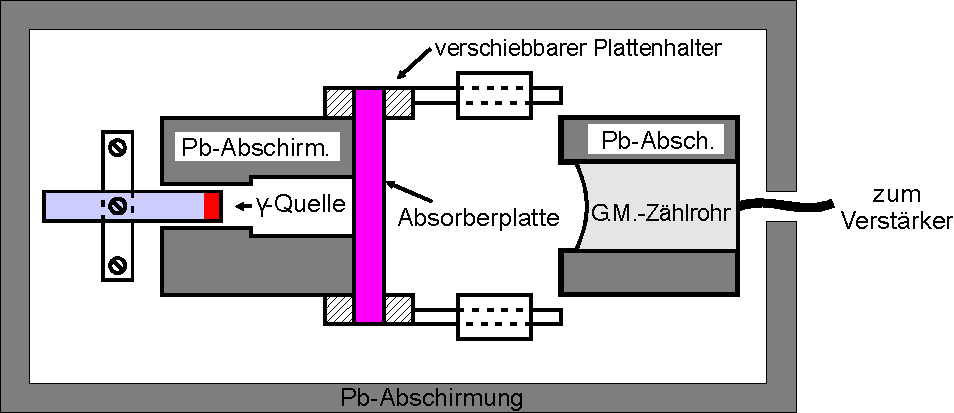
\includegraphics{figures/abb7.pdf}
    \caption{Schematische Darstellung der verwendeten Messaperatur \cite{ap04}.} 
    \label{fig:schemaaufbau}
\end{figure}